\documentclass[11pt]{article}
\usepackage[margin=1in]{geometry}
\usepackage[T1]{fontenc}
\usepackage{lmodern}
\usepackage{microtype}
\usepackage{amsmath}
\usepackage{booktabs}
\usepackage{tabularx}
\usepackage{xcolor}
\usepackage{pgfplots}
\pgfplotsset{compat=1.18}
\usepackage{enumitem}
\setlist{itemsep=2pt,topsep=4pt}
\usepackage[hidelinks]{hyperref}

\newcommand{\code}[1]{\texttt{#1}}

\title{Exact, Output-Identical Acceleration of MAFFT\\across CPU Architectures and GPUs}
\author{Claude Code (Claude Opus 5.5, Anthropic)\thanks{Claude Code, running Claude Opus 5.5,
designed, implemented, verified and benchmarked the optimizations and wrote this report; the
three opt7 workstreams were carried out by parallel Claude Code agents. Josh Walker advised and
set the research direction. The dikarya1 build (Section~\ref{sec:dikarya}) was made by Claude
Code under the direction of Alan Rockefeller.} \and Josh Walker}
\date{Technical report, September--October 2026}

\begin{document}
\maketitle

\begin{abstract}
We describe a series of builds of the multiple sequence aligner MAFFT 7.526 that run faster
while producing output \emph{byte-identical} to unmodified MAFFT, so that downstream analyses
calibrated on stock output are unaffected. The first four builds targeted an Apple M1. They
found that much of the run time of the accurate L-INS-i mode went not to the
dynamic-programming (DP) recurrences but to bookkeeping, added a pair-score cache for
iterative refinement, and moved the all-pairs local-alignment stage to the GPU with an integer
Metal kernel that reproduces MAFFT's recurrence, tie rules and traceback exactly. The fifth
ported the vector kernels to AVX-512 and exposed that \emph{stock MAFFT itself} does not give
the same alignments on every platform: a gcc build on x86 disagrees with the Mac on a third of
inputs, because Apple's clang fuses multiply-adds and gcc does not, while a clang build with
FMA on x86 reproduces the Mac's alignments. ``Identical to stock'' must therefore name the
stock build's rounding class.

A build directed by Alan Rockefeller for Dikarya, a web service running on an AVX2 server
without AVX-512 (dikarya1), contributed an integer
local-alignment fill that stores markers in place of gap offsets and recovers them during
traceback. It was faster on AVX-512 too (opt6), and prompted a broader exploration. For opt7,
three AI agents worked in parallel, one per architecture (AWS Graviton, AMD Zen~5 and Intel
Granite Rapids, and an NVIDIA GPU), from the same tree and under the same exactness contract.
Without communicating, they arrived at several of the same techniques, each written for its own
platform. opt8 consolidated their work into one tree in which most code is portable and shared,
and carrying each workstream's techniques to the other platforms made every machine we measured
faster than opt7: 1.35$\times$ on AMD Zen~4 and Intel Sapphire Rapids with unchanged build
flags, 1.24$\times$ for the AVX2 server's build class, 1.22$\times$ on the M1 and 1.05$\times$ on
Graviton4. On production fungal ITS alignments, L-INS-i now runs 8.1$\times$ faster than stock in
a single run on the M1 (5.1$\times$ at eight concurrent), 7.5--9.8$\times$ faster at four concurrent alignments on recent AWS x86
instances, about 5$\times$ on Graviton, and 5.9$\times$ on an AVX2-only host. A CUDA port of the
GPU stage adds 1.24$\times$ but does not pay on AWS. Every output of every build in every test
was byte-identical to its stock reference; the one discrepancy the work introduced, a rounding
difference in opt1, was caught by independent validation and fixed.
\end{abstract}

\section{Introduction}

MAFFT~\cite{katoh2002,katoh2013} is among the most widely used multiple sequence aligners.
Its iterative-refinement modes with pairwise alignment information, notably L-INS-i and
G-INS-i~\cite{katoh2005}, are considerably more accurate than its progressive modes, but
also much slower. This work was prompted by a concrete cost: a phylogenetics pipeline
(``seqhesion'') aligns 2{,}415 fungal ITS barcode sets per genomic region with L-INS-i, at
roughly 80--95\,s each, and MAFFT is about 99\% of the pipeline's run time.

Faster aligners exist, but they change the answer. The pipeline's own measurements, taken
by comparing well-supported splits of FastTree~\cite{price2010} trees built after
trimAl~\cite{capella2009} trimming, found that MAFFT FFT-NS-1 (135$\times$ faster) recovers
78.3\% of the splits supported in the L-INS-i trees, and spoa~\cite{vaser2017} recovers
69.7\%. We therefore set a stricter goal: make L-INS-i faster \emph{without changing a single
output byte}. Such a speedup costs nothing in accuracy and needs no revalidation downstream.

The work proceeded in a series of builds, each verified before use
(Table~\ref{tab:builds}). Each reports a version string of the form \code{7.526-opt}$N$ so
that downstream caches and provenance records can tell them apart
(Section~\ref{sec:provenance}).

The first four builds target the M1. The fifth followed when the pipeline, now running the
same L-INS-i recipe over a much larger corpus, moved to AWS Batch, and the instance type had to be chosen on measured cost. Porting the vector kernels to
x86 was routine (Section~\ref{sec:opt5}). The exactness criterion was not. ``Byte-identical to
stock'' turned out to depend on how stock was compiled: stock MAFFT built with gcc on x86
gives different alignments from stock MAFFT on the Mac for a third of the inputs, and only a
build that fuses multiply-adds the way Apple's compiler does agrees with it
(Section~\ref{sec:xplat}).

After the series was published, Alan Rockefeller directed a build for the AVX2-only server of
the Dikarya web service (dikarya1, Section~\ref{sec:dikarya}), which contributed a new local-alignment fill that also made our own x86
build faster (opt6). That prompted a broader experiment: three AI agents, one per architecture,
optimizing in parallel under the same contract (opt7, Section~\ref{sec:opt7}), followed by a
consolidation of their work into one shared, mostly portable tree (opt8,
Section~\ref{sec:opt8}). The agents arrived independently at several of the same techniques, and
sharing them across platforms made every platform faster.

\begin{table}[h]
\centering
\caption{The builds, as commits on top of upstream MAFFT 7.526 (sizes are \code{core/} only).}
\label{tab:builds}
\begin{tabularx}{\linewidth}{llX}
\toprule
Build & Size & Content \\
\midrule
opt1 & 8 files, +1197/$-$147 & Bookkeeping fixes, NEON DP rows, GEMM-based scores (Section~\ref{sec:round1}) \\
opt2 & 5 files, +380/$-$96 & Refinement pair-score cache, vector prefix scan, run-based counts (Section~\ref{sec:round2}) \\
opt3 & 4 files, +554/$-$10 & All-pairs local alignment on the GPU with Metal (Section~\ref{sec:gpu}) \\
opt4 & 4 files, +230/$-$146 & Shader compiled at build time; occupancy-tuned kernel (Section~\ref{sec:opt4}) \\
opt5 & 7 files, +505/$-$29 & AVX-512 kernels for x86; multiply-add rounding matched to each platform's stock build (Section~\ref{sec:opt5}) \\
dikarya1 & 11 files, +659/$-$18 & AVX2 paths for x86 without AVX-512: marker fill, sparse profile scores, uncleared work rows (Section~\ref{sec:dikarya}) \\
opt6 & 1 line & dikarya1's marker fill on AVX-512 builds (Section~\ref{sec:dikarya}) \\
opt7 & 11 files, +2513/$-$38 & Linux arm64, newer x86 AVX-512 and CUDA, from three parallel workstreams (Section~\ref{sec:opt7}) \\
opt8 & 12 files, +574/$-$1383 & Consolidation into shared, portable code (Section~\ref{sec:opt8}) \\
\bottomrule
\end{tabularx}
\end{table}

\section{Setting and methodology}

\paragraph{Hardware.} Apple M1 (4 performance + 4 efficiency cores), 16\,GB, 128-bit NEON
SIMD, and the undocumented AMX matrix coprocessor reachable through Apple's Accelerate
BLAS, and an 8-core GPU. Compiler: Apple clang 21, \code{-O3}. The machine was upgraded
from macOS 26.6 to macOS 27.0 between opt3 and opt4; opt4 is the first build compiled with
the macOS 27 toolchain (Section~\ref{sec:os}).

\paragraph{x86 hardware.} For opt5, one AWS instance running Amazon Linux 2023 (glibc 2.34),
first as a c7i.xlarge (Intel Xeon Platinum 8488C, Sapphire Rapids: 2 cores with 2 hyperthreads
each, AVX-512, 105\,MB L3) and later, on the same disk, as a c7a.xlarge (AMD EPYC 9R14,
Zen~4: 4 cores without SMT, AVX-512, 16\,MB L3). Compilers: gcc 11.5 and clang 15.0.7 from the
distribution. Stock references were built on the instance from the upstream v7.526 tag.

\paragraph{More architectures.} From dikarya1 on: the Dikarya host (Section~\ref{sec:dikarya});
and on AWS, all xlarge (4 vCPUs) with Amazon Linux 2023, clang 15 and gcc 11: c8a (AMD EPYC,
Zen~5), c8i (Intel Xeon, Granite Rapids), c8g (Graviton4, Neoverse V2, 128-bit SVE2), c7g
(Graviton3, Neoverse V1, 256-bit SVE), g6 (NVIDIA L4; host AMD EPYC 7R13, Zen~3, AVX2 without
AVX-512) and g4dn (NVIDIA T4; host Intel Cascade Lake), plus the c7a and c7i of opt5.

\paragraph{Workloads.}
(i)~Production ITS alignments: about 180 sequences of 500--1200\,bp with ragged,
indel-rich ends, giving aligned widths near 2{,}000 columns; run with
\code{-{}-localpair -{}-maxiterate 1000 -{}-thread 1}.
(ii)~Synthetic protein and DNA families generated along random trees with substitutions and
indels (100--3{,}000 sequences; a 480-sequence DNA set for large groups).
(iii)~MAFFT's bundled test files.
(iv)~The pipeline's full corpus: two genomic regions with 2{,}415 and 1{,}723 production
shards, plus 205 larger ``targeted'' windows of 64--532 sequences, each with a stored
reference alignment. These alignments are about 71\% gaps, which matters for exactness
testing: gap-rich alignments produce near-ties, and near-ties are what expose rounding
differences. A synthetic family, by contrast, aligned with only 8\% gaps.

\paragraph{Measurement.} The machine carried unrelated background load for most of the
session, so wall-clock time was unreliable. We used (a)~statistical profiles from macOS
\code{sample}, attached to each MAFFT stage binary as it started, and (b)~per-stage retired
instructions and elapsed cycles from \code{/usr/bin/time -l}, via wrapper binaries. Cycle
counts are less sensitive than wall time to other load but not immune to it, since cache
and memory contention still inflate them, so comparisons were run side by side where possible. Final
wall-clock benchmarks were taken on a quieter machine (Section~\ref{sec:results}).

\paragraph{Exactness criterion.} Every change must leave final alignments byte-identical to
stock MAFFT with \code{-{}-thread 1}. Stock MAFFT's multithreaded refinement is itself
nondeterministic: two runs of an unmodified build with \code{-{}-thread 4} produced different
alignments. Single-thread runs are deterministic, and those were compared. ``Stock'' means
upstream MAFFT compiled for, and run on, the same platform as the optimized build; on the M1
that is Homebrew's 7.526, built with Apple clang. Section~\ref{sec:xplat} shows why the
compiler belongs in that definition.

\section{Round 1 (opt1): removing bookkeeping}
\label{sec:round1}

\subsection{Where the time went}

MAFFT runs as a pipeline of separate stage programs. For L-INS-i on a 180-sequence ITS set,
about 25\,s was spent in \code{tbfast} (all-pairs local alignment) and about 60\,s in
\code{dvtditr} (tree-dependent iterative refinement). Inside \code{dvtditr}, the DP itself
(\code{partA\_\_align}) accounted for only about 13\% of samples. The largest single
consumer, 54\%, was \code{fillimp}, which builds the ``importance'' matrix encoding the
pairwise local-alignment hints. Most of that time went to its helper \code{movereg}, which
converts residue indices to alignment columns by rescanning each gapped sequence from the
start, once per hint segment per sequence pair, on every refinement step. Other significant
costs were zeroing the dense importance matrix (${\sim}2{,}000^2$ doubles, 32\,MB) on every
call, column-major loops over 180 rows (\code{commongappick\_record}, traceback output,
profile construction), and the intergroup sum-of-pairs score.

For FFT-NS-2 on 3{,}000 proteins, 64\% of samples were in \code{naivepairscorefast}, the
per-pair distance computed from the first-pass alignment, followed by the progressive DP
\code{A\_\_align} (${\sim}20\%$).

\subsection{Principles for exact rewrites}
\label{sec:principles}

Floating-point results depend on the order of operations, so ``the same algorithm, faster''
is not automatically byte-identical. Four observations made exact rewrites possible:

\begin{enumerate}
\item \textbf{Integer-valued arithmetic.} In default L-INS-i the scoring matrices are
  \code{int} scaled by $1.0$, penalties are integers, and the score offset is zero. Every
  value in the \code{double} DP is therefore an integer far below $2^{53}$. An \code{int32}
  DP makes exactly the same comparisons, and integer sums may be reordered freely. A
  runtime guard checks integrality and range, and falls back to the original code if the
  check fails.
\item \textbf{Matching fused multiply-add contraction.} Clang contracts expressions of the
  form $a + b\cdot c$ into a single-rounding \code{fmadd}. We inspected the stock binaries'
  disassembly and reproduced each contraction with explicit \code{fma()} or
  \code{vfmaq\_f64}. Getting this wrong in one place produced the only discrepancy of the
  project (Section~\ref{sec:bug}). This contraction is a property of the compiler, not of
  MAFFT: other compilers and targets round the same source differently, so opt5 makes the
  choice per platform (Sections~\ref{sec:opt5} and~\ref{sec:xplat}).
\item \textbf{Order-preserving accumulation.} Where non-integer values are accumulated,
  such as profile construction, gap frequencies, and the weighted intergroup total, loops
  were restructured (for example, from column-major to row-major) so that each accumulator
  still receives its terms in the original order.
\item \textbf{Associative scans with the original tie rule.} In the DP rows, the horizontal
  gap state is a running maximum. A running maximum is exact in any evaluation order,
  provided ties keep the position the original chose (the earlier one for \code{>}, the
  later one for \code{>=}). The only wrinkle is the zero-extension-penalty case
  $m \leftarrow \max(\cdot) + 0.0$. Adding $0.0$ only maps $-0$ to $+0$ and never changes
  a comparison, so it can be applied once after the scan.
\end{enumerate}

\subsection{Optimizations}

\paragraph{1. Residue-to-column maps in \code{fillimp}.} Before scanning the hint segments,
we build, for each sequence, the alignment column of each residue. Converting a segment
boundary is then a lookup, and walking a segment becomes a branch-free loop
$\mathit{imp}[p_1(s_1{+}n)][p_2(s_2{+}n)] \mathrel{+}= w$ that visits the same cells in the
same order as the original pointer walk. This reduced \code{fillimp} samples from about
13{,}400 to about 1{,}000.

\paragraph{2. Integer NEON kernel for \code{L\_\_align11}.} Under the integrality
precondition, the local-alignment fill runs in \code{int32}. In MAFFT's formulation, every
candidate for cell $(i,j)$ is derived from row $i{-}1$. A row therefore needs only one
scalar prefix scan for the horizontal-gap state, rewritten as
$H_j = (j{-}1)e + \max_{k\le j-2}(p_k - k e)$ with first-occurrence arg-max, followed by a
branch-free loop over $j$ in \code{int32x4} NEON vectors. This covers the gap candidates,
vertical state, traceback codes, row maximum, and local-threshold clamp. The substitution
scores come from a per-call query profile. Cells that the original leaves stale (the last
row and column) are provably write-only, so they need not be reproduced. The kernel was
4.3$\times$ faster by samples, and \code{tbfast} fell from 99.3G to about 22G cycles.

\paragraph{3. Sparse zeroing of the importance matrix.} The matrix is zeroed in full once
per allocation. After that, \code{fillimp} records the range of columns it writes in each
row, and the next call zeroes only those ranges. RNA mode, which also writes the matrix,
resets this state. Samples for \code{memset} fell from about 1{,}900 to about 140.

\paragraph{4. Closed-form intergroup score, via GEMM.} The per-pair loop in
\code{intergroup\_score} is a state machine over gap runs. We showed that its result equals
the substitution sum over columns where neither sequence has a gap, plus, for each maximal
gap stretch in one sequence, a penalty and an extension term anchored at the first column
of that stretch where the other sequence has a residue. The gap terms reduce to a few
lookups per stretch. The column sums for all pairs at once form an integer matrix product
$T = XY^{\top}$, where $X$ is a one-hot encoding of group~1's letters and $Y$ holds group~2's
scores against each letter. We evaluate $T$ with Accelerate's \code{cblas\_sgemm}, using
\code{float32} only when every partial sum stays below $2^{24}$ and \code{float64}
otherwise, and add rare letters as sparse corrections. For small groups a direct
\code{int32} loop is cheaper and is used instead. The weighted total is still accumulated
pair by pair in the original order.

\paragraph{5. Row-major rewrites.} \code{commongappick\_record}, \code{gapcountf}, and the
column profiles in \code{alignableReagion} now walk each sequence contiguously while
preserving the per-column order of additions. The traceback first records the path as two
index lists, then writes each of the $\sim$180 output rows contiguously, instead of
touching every row for each column. Traceback samples fell from about 1{,}040 to about 220.

\paragraph{6. NEON row kernels for the profile DPs.} In \code{partA\_\_align} (refinement)
\code{USE\_PENALTY\_EX} is 0. In \code{A\_\_align} (progressive), the extension penalty
defaults to $0.0$. In both cases the horizontal state is a pure running maximum
(Section~\ref{sec:principles}). Each row is computed as a scalar max-scan followed by a
\code{float64x2} loop whose \code{vfmaq\_f64} operations reproduce the stock \code{fmadd}s
exactly. \code{A\_\_align} falls back to the original loop when the extension penalty is
nonzero or when shifted alignment (\code{trywarp}) is enabled.

\paragraph{7. Pattern-grouped substitution profiles.} In the refinement DP the costliest
part turned out to be \code{match\_calc}, which rebuilds each row's substitution scores by
walking per-column lists of nonzero profile entries. We group the columns of the second
profile by their ordered pattern of nonzero letters. Within a group every column uses the
same per-row scalars, so each group becomes a short vector loop with the identical
\code{fma} sequence.

\paragraph{8. All-pairs MSA distances for FFT-NS-2.} \code{naivepairscorefast} discards
columns where both sequences have a gap, then adds substitution scores and one penalty per
gap run. A maximal gap stretch in $s_1$ becomes one such run exactly when $s_2$ has a
residue inside it, so the run count needs only prefix-count lookups per stretch. The
substitution sums for all $N^2/2$ pairs are computed as GEMM tiles over
(rows $\times$ columns $\times$ alignment-column chunks), which keeps memory bounded even for
very gappy alignments (5{,}515 columns for 350-residue sequences in one test). All
4{,}498{,}500 distances for 3{,}000 sequences matched the original bit for bit.

\section{Round 2 (opt2): measuring refinement}
\label{sec:round2}

After opt1, a 180-sequence ITS shard spent about 22\,G cycles in \code{tbfast} and 54\,G in
\code{dvtditr}. Rather than guess at the next target, we instrumented a copy of the
refinement loop to record, for every step, its outcome and where its time went.

\paragraph{How refinement behaves.} With \code{-{}-thread 1}, MAFFT runs refinement through
its threaded code path with a single worker: each ``generation'' realigns the two sides of
every tree branch (about 355 branches here) against the current alignment and keeps a
realignment only if it improves the objective. Shards converged in 5--8 generations. About
85\% of branch steps reproduced the existing alignment exactly, about 3\% were accepted
and the rest were rejected. Time within a step split roughly 16\% scoring before the
realignment (\code{intergroup\_score}), 16\% building the importance matrix, and 64\% in the
realignment itself.

Two caching ideas followed from this, and only one survived measurement. Memoizing a whole
branch step is useless (at most 2\% of steps could reuse a previous result): the
realignment's input is the full alignment, uncompacted, and every accepted step changes it.
But the score computed before each realignment is a weighted sum of per-pair scores, and a
pair's score depends only on its two rows. Between acceptances the rows do not change, so
89--95\% of the pair scores requested had already been computed on identical rows.

\paragraph{1. Pair-score cache.} Each refinement thread keeps a snapshot of every row and a
version number that changes whenever the row's text changes, detected by comparing each
row with its snapshot. A cached pair score is reused only when it was computed on the
current versions of both rows. Per-pair scores are exact integers (Section~\ref{sec:principles}),
so how they were computed does not matter; the weighted total is still accumulated in the
original order. Misses are computed in two blocks using the opt1 scoring kernel. The
$n^2$ table is allocated on first use and the cache disables itself above 32\,MB per thread.
This cut \code{dvtditr} cycles by 11--13\%.

\paragraph{2. Vector prefix scan in \code{L\_\_align11}.} Profiling split out of the opt1
kernel showed its scalar prefix scan cost as much as the whole NEON loop: the scan's
compare-and-select chain limits it to about two cycles per cell. A running maximum with
first-occurrence arg-max is two prefix maxima --- one of the values, and one of the
positions where a value strictly beats everything before it --- so both can be computed
four lanes at a time with two log-step scans and a carry between blocks. Fused into the
main NEON loop, this removed a third of \code{tbfast}'s instructions and 18--19\% of its
cycles. Two alternatives were slower: fusing the next row's \emph{scalar} scan into the
vector loop (+16\% cycles, as it degraded code generation) and unrolling the vector scan
over two blocks (no gain; the loop was already throughput-bound).

\paragraph{3. Gap runs instead of columns.} The per-column gap-opening, gap-closing and
gap-frequency counts used in every profile DP tested every column of every row with a
branch. Since each column receives $\mathit{eff}_j$ from rows in ascending order however
the loop is structured, we find each row's gap runs sixteen bytes at a time with NEON and
visit only the columns where runs start, end or lie.

\paragraph{4. Compact anchor profiles.} \code{alignableReagion} zeroed two
26-letter profiles of the full alignment length, about 0.8\,MB, on every call. It now
reuses a buffer and keeps only the letters present, visiting nonzero bins in the same
descending order so that the site scores are identical. We checked the compiled floating-point
instruction mix against the original and compared the scores per call.

Together, side by side with opt1: 28--30\% fewer instructions and 16--18\% fewer cycles.

\section{opt3: the all-pairs stage on the GPU}
\label{sec:gpu}

After opt2, \code{tbfast}'s all-pairs local alignment was about a third of all cycles: 4.6--5.8
billion DP cells per shard at about 4.4 cycles per cell. The M1's GPU sat idle, and the
pipeline already occupies every CPU core with separate inputs, so moving this stage off
the CPU frees capacity rather than competing for it.

\paragraph{Mapping.} In MAFFT's formulation, row $i$ of the local-alignment DP depends only
on row $i{-}1$. We assign one pair to each 32-lane SIMD group. Each lane owns a contiguous
run of $C = \lceil \ell_2/32\rceil$ columns and holds, per column, the previous row's value,
the vertical-gap state and the second sequence's residue code. The horizontal-gap state
needs a prefix maximum across the whole row: each lane scans its own columns, and one
SIMD-wide scan of the lane totals, built from \code{simd\_shuffle\_up}, carries the maximum
and its first-occurrence position across lanes. The row maximum and its first column are
two SIMD reductions. The traceback matrix is stored as \code{int16} in GPU memory, laid out
lane-interleaved so that each store instruction writes one contiguous 64-byte span; this
alone saved 14\% of GPU time. After the fill, one lane walks the traceback exactly as
MAFFT's \code{Ltracking} does and writes the two aligned strings, so the CPU receives only
results.

\paragraph{Exactness.} The kernel uses only \code{int32} arithmetic, the same comparisons,
and the same tie rules as the CPU kernel, so exactness does not depend on the GPU's
floating-point behavior at all. The host sends a pair only when every precondition of the
CPU integer kernel holds --- integral scores, every character in the scoring alphabet,
the \code{int32} range bound --- and when the second sequence is 64--2{,}048 residues.
Anything else, or any GPU failure, takes the unchanged CPU path. \code{MAFFT\_NOGPU=1}
disables the GPU entirely, which proved useful for isolating the GPU stage in testing.

\paragraph{Integration.} Before its pair loop, \code{pairalign()} sends every eligible pair to
the GPU in batches of about 96\,MB of traceback memory, two batches in flight; the pair loop
then copies stored results instead of calling \code{L\_\_align11}. The CPU thread waits
rather than spins, so the stage's CPU time fell from 5.6\,s to 0.6\,s per shard and its
wall time from 5.7\,s to 1.8\,s.

\section{opt4: build-time shader compilation and occupancy}
\label{sec:opt4}

\paragraph{Build-time compilation.} opt3 compiled its shader from embedded source when it ran.
In opt4 the kernel is a template in its own source file, instantiated for each column
count per lane, and compiled at build time into a Metal library embedded in the binary.
If the build machine has no Metal compiler, the embedded source is compiled at run time
as before, and a library that fails to load also falls back to the source. This pins the
front-end compile (source to Metal's intermediate representation, AIR), which an OS update
could otherwise change. The final compile from AIR to GPU machine code still happens in
the driver at run time, so OS dependence is narrowed, not removed.

\paragraph{Occupancy.} Forcing wider kernel variants for the same data showed the kernel was
limited by occupancy (Table~\ref{tab:occupancy}): each lane's columns were held in registers,
capping pipelines at 384 threads per threadgroup, and GPU time grew steeply with the column
count per lane until, at 48 columns, the compiler gave up on registers and time dropped.
Looping to the actual column count instead of the compile-time maximum makes the compiler
keep those arrays in thread memory, raising the cap to 832--896 threads per threadgroup.
Packing four pairs into each threadgroup helped a further 8\%, and dropping the variants below
20 columns per lane, which the compiler still kept in registers, made one shard 20\% faster.

\begin{table}[h]
\centering
\caption{GPU time for all 16{,}110 pairs of one shard (c0.0001) on macOS 27, by where
each lane's column state lives.}
\label{tab:occupancy}
\begin{tabular}{lrr}
\toprule
Kernel & Columns per lane & GPU time \\
\midrule
Registers (opt3) & 20 & 2.47\,s \\
                 & 24 & 3.82\,s \\
                 & 32 & 5.09\,s \\
                 & 48 (compiler spills) & 2.00\,s \\
Thread memory, loop to actual count & 20 & 1.26\,s \\
\quad + four pairs per threadgroup (opt4) & 20 & 1.20--1.23\,s \\
\bottomrule
\end{tabular}
\end{table}

\paragraph{The OS upgrade.} On macOS 27 the unchanged opt3 kernel ran about 40--50\% slower
than on macOS 26 (2.3--2.46\,s against 1.67\,s for one shard). Every variant we tried was
affected equally, so the change came with the OS, from the GPU compiler, driver, or the
thermal state of this fanless machine. opt4's tuning more than recovers it.
\label{sec:os}

\section{opt5: x86-64 with AVX-512}
\label{sec:opt5}

opt5 is opt4 plus x86 back-ends. The arm64 build is unaffected: compiled with Apple clang,
all 32 opt5 binaries have the same instruction streams as opt4's, differing only in the
version string, and they gave identical outputs and timings to opt4 on the M1.

\paragraph{Multiply-add rounding per platform.} opt4 called \code{fma()} in 15 places to
reproduce Apple clang's contraction of the stock expressions (Section~\ref{sec:principles}).
On x86 those calls would be wrong. The reference build there, upstream compiled with gcc and
\code{-std=c99}, never contracts (gcc disables contraction in ISO C mode), and the x86-64
baseline has no FMA instruction at all. The binaries of the conda-forge package of 7.526
contain none either. opt5 therefore writes these sites as
\code{MULADD(a,b,c)}, which is \code{fma(a,b,c)} where the stock build fuses (clang on arm64)
and \code{a*b+c} otherwise; a build-time switch, \code{MAFFT\_STOCK\_FMA}, overrides the
choice. The NEON blocks that use \code{vfmaq\_f64} are compiled only when fusion is on. A
gcc build of opt5 with AVX-512 enabled was checked to contain no FMA instructions.
Section~\ref{sec:xplat} returns to which rounding the x86 reference should use.

\paragraph{Profile on x86.} With no GPU, the all-pairs stage stays on the CPU, so the x86
profile differs from the M1's. With only the \code{L\_\_align11} fill ported, a production
shard spent 23\% of samples in \code{partA\_\_align}, 16\% in the integer local-alignment
fill, 14\% in \code{fillimp}, 11\% in \code{match\_calc}'s grouped profiles, and 6\% in
\code{alignableReagion}, with the rest spread over gap counting, column compaction and pair
scoring. These measurements were taken while a four-process stock run occupied the machine,
so the times are relative only: through the changes below, except the column compaction
and the pair-sum gather, which came last, one shard went from 40.2\,s to 29.9\,s.

\paragraph{1. Integer local-alignment fill, 16 cells at a time.} The opt2 NEON row kernel
(fill plus both prefix scans) was ported to AVX-512 at sixteen \code{int32} lanes, with
\code{valignd} providing the lane shifts for the log-step scans, and to SSE4.1 lane for lane.
Once the fill ran sixteen cells per step, a third of the function's samples landed on one
scalar loop: when a row's maximum beats the best so far, the original searches the row for
the first cell holding it. That search now compares sixteen cells per step and takes the
first match.

\paragraph{2. Profile DP rows at eight doubles.} The NEON row fills of \code{partA\_\_align}
and \code{A\_\_align} became eight-lane AVX-512 loops whose multiply-adds go through a vector
form of \code{MULADD}. The running best of the horizontal-gap state, still a scalar loop in
opt4, is now an eight-lane prefix scan over (value, position) pairs. ``Replace the earlier
pair only if the later value is strictly greater'' (or ``greater or equal'' in
\code{A\_\_align}) is associative, so three shift-compare-blend steps plus a carry give each
lane exactly the scalar result. Blends rather than \code{max} keep ties between $-0$ and $+0$
as the scalar code resolves them.

\paragraph{3. Gathers and scatters.} The refinement adds the importance matrix into each row
through a column map; this is now an AVX-512 gather. In the grouped substitution profiles,
the per-row score table is computed eight letters at a time (each letter's sum still runs
over the alphabet in order), and each column group is computed eight columns at a time and
written back with a scatter. The per-pair \code{int32} sums used for the refinement's pair
scores, which ran through Accelerate's GEMM on the Mac but fell back to a scalar loop on x86,
use a sixteen-lane gather; integer sums may be reordered freely.

\paragraph{4. Byte masks.} Gap runs are found 64 bytes at a time: one compare gives a 64-bit
mask $g$ of gap positions, and $g \oplus (g \ll 1 \,|\, \mathit{carry})$ marks every run
boundary, visited in order with count-trailing-zeros. \code{alignableReagion}'s profile pass
visits only non-gap bytes (production alignments are about 71\% gaps), in the same order, so
each bin receives the same additions. Its character-presence pass pre-marks a few common
characters whose bins are valid and visits only the remaining bytes; an extra valid
character can only add an all-zero bin, which the site score skips. Column compaction moves
runs of kept columns with \code{memmove} instead of copying single bytes.

\paragraph{What did not help on Sapphire Rapids.} The importance-matrix fill
(Section~\ref{sec:round1}, item~1) was the obvious next target: about 22\% of samples and
1.7 billion scattered updates per shard. Walking all segments over one band of 32 rows at a
time keeps the per-cell order of updates, and therefore the result, but was slower, even
with segments bucketed by band to avoid revisiting them. Software prefetching a few cells
ahead in each segment did not help either (58.7--60.0\,G cycles per shard without it,
60.5--62.2\,G with it). The c7i's 105\,MB
L3 holds the whole 32\,MB matrix, and the out-of-order core already overlaps the misses.
Both were dropped here. Banding later paid on Graviton, whose L2 holds a band, and opt8 uses
it on every platform (Sections~\ref{sec:opt7} and~\ref{sec:opt8}).

\paragraph{Verification.} Each rewritten function got a per-call harness in the style of
Section~\ref{sec:verify}: a patch that runs the vector and the scalar path on the same
inputs on every call and aborts on any bitwise difference, covering the row fills and scans,
the grouped profiles, the anchor profiles, the gap runs, the column compaction and the pair
sums. They ran under L-INS-i (default and changed \code{-{}-lop}/\code{-{}-lexp}), G-INS-i,
E-INS-i and FFT-NS-2, on DNA and on the bundled protein sample, with every end-to-end
output also compared with stock, under both the gcc build and the clang+FMA build of
Section~\ref{sec:xplat}.

\section{Identical to which stock?}
\label{sec:xplat}

The acceptance rule for the AWS deployment came from the pipeline: an optimized build must
be byte-identical to stock 7.526 built and run on the same instance. The natural reference is
upstream built with its own Makefile, i.e.\ gcc \code{-O3 -std=c99}. The conda-forge binary
gave the same output on the shards compared and ran about 7\% slower. The test set had 183
shards (181 distinct inputs; some shard names share an input). It comprised the pipeline's
13-window canary (the largest leaf and rung-1 shards of both regions, plus the shard of
Section~\ref{sec:bug}), the first 100 production shards of one region, its 40 largest targeted
windows (217--532 sequences), and 30 shards from three components of the pipeline's current build.
Each has an alignment stored on the Mac.

\paragraph{The gcc build disagrees with the Mac.} The gcc stock build matched the stored Mac
alignments on only 122 of 181 inputs (Table~\ref{tab:xplat}). The differences are mostly not
one-residue ties. Aligned widths differ by up to about 60 columns (for example 2{,}028
against 1{,}997 for one production shard), consistent with refinement taking a different path
after an early near-tie; a few inputs differ by one to seven residues. The large targeted
windows, with the most near-ties, diverge most often.

\begin{table}[h]
\centering
\caption{Stock MAFFT 7.526 on x86 against the alignments stored on the Mac (Apple clang,
arm64): distinct inputs with byte-identical L-INS-i output, \code{-{}-thread 1}.}
\label{tab:xplat}
\begin{tabular}{lrrr}
\toprule
Set & Inputs & gcc \code{-O3} & clang \code{-O3 -march=x86-64-v3} \\
\midrule
Canary windows & 11 & 7 & 11 \\
Production shards & 100 & 75 & 100 \\
Targeted windows (217--532 seqs) & 40 & 15 & 40 \\
Current-build shards & 30 & 25 & 30 \\
\midrule
Total & 181 & 122 (67\%) & 181 (100\%) \\
\bottomrule
\end{tabular}
\end{table}

\paragraph{The cause is multiply-add contraction.} Apple's clang, like clang generally,
contracts $a\cdot b + c$ within an expression into a fused multiply-add rounded once
(\code{-ffp-contract=on} is its default); gcc in ISO C mode does not contract, and the x86-64
baseline target has no FMA instruction anyway. Clang applies its contraction rule in the front
end, independently of the target, so stock MAFFT built with clang for an x86 target that has
FMA (\code{-march=x86-64-v3}) fuses the same expressions as the Mac build. That build
reproduced the Mac's alignments on all 181 inputs. On this set, then, the platform difference
is entirely the rounding of multiply-adds, and no other source of difference, system
libraries included, showed up, in line with the library-independence argument of
Section~\ref{sec:verify}.

\paragraph{Choosing the reference.} Neither rounding is more correct; they only break
near-ties differently. The pipeline's maintainer therefore chose on speed and on whether
results could be shared between the Mac and AWS. Clang+FMA was slightly faster, by 2--6\%
for both stock and opt5 (Table~\ref{tab:x86four}), and it lets the alignment cache be shared.
The AWS reference is therefore stock 7.526 built with clang and FMA, and the production build is
opt5 compiled the same way with \code{-march=x86-64-v4 -DMAFFT\_STOCK\_FMA=1}. Under that
build opt5's own multiply-adds fuse, and its vector loops use FMA instructions to match. It
was accepted against the clang reference on all 183 shards, run on the same instance, on
both instance types.

\paragraph{Intel and AMD agree.} Rebuilt natively on the c7a, all four builds (gcc and clang
stock, gcc and clang opt5) produced stage binaries byte-identical to the c7i builds, and the
outputs agreed between the two machines wherever compared: all 183 shards for clang stock and
both opt5 builds, and the canary windows for gcc stock.

\paragraph{Placement.} The pipeline also places new sequences into stored shard
alignments with \code{-{}-add} or \code{-{}-addfragments} and \code{-{}-keeplength}, a
progressive path rather than L-INS-i. A 12-case canary of real placements gave identical
output for every build: Homebrew stock, opt4 and opt5 on the Mac, and gcc and clang stock and
opt5 on the c7a. This was also the first byte-level check of opt4 on that invocation.

\paragraph{Trees.} The pipeline goes on to trim with trimAl \code{-gappyout} and build trees
with FastTree \code{-gtr -gamma -nt}. trimAl 1.5.1, built on x86, reproduced the Mac's
trimmed alignments for all 183 shards. FastTree did not reproduce the Mac's trees: starting
from the Mac's own alignments, only 3 of 183 trees were byte-identical. Bioconda compiles
FastTree with \code{-O3 -funsafe-math-optimizations} on both platforms, which allows the
compiler to reassociate floating-point sums, so its output depends on the compiler and the
vector width. Two x86 builds of the same source (bioconda's binary, from gcc 13, and a
gcc 11 build) disagreed with each other as well. Within AWS, the same binary gave
identical trees on the c7i and the c7a for all 183 shards.

How much the tree differences matter depends on how the trees are used. The pipeline roots each
tree on its scaffold, prunes the scaffold, and collapses internal branches shorter than half
an expected substitution, $0.5/w$ for trimmed width $w$ (about $10^{-3}$). Compared that way,
the x86 trees from the bioconda binary matched the Mac's in 132 of 183 shards (72\%). In 37
more (20\%) the only differences were groups of tips (up to 31) with near-zero branches
sitting on the other side of a branch of identical length: likelihood ties broken
differently. In 14 (8\%) there were other differences, with symmetric differences of 2--13
kept splits. Branch lengths on shared splits agreed to within $3\times10^{-3}$. The pipeline
measured the end-to-end effect itself, rebuilding one component's 548 trees with a different
FastTree build. Its coarse hierarchy levels were unchanged, finer levels had adjusted Rand
indices of 0.983--0.997, and 95.5\% of groups were unchanged, about a sixth of the change
caused by re-sampling its input cover. It now shares alignments between the Mac and AWS and
computes trees per platform; trees cost about a second each against 20--100\,s for the alignment.

\section{dikarya1 and opt6: a server without AVX-512}
\label{sec:dikarya}

The opt5 kernels need AVX-512. On x86 CPUs without it, which include every Intel server part
before Skylake-SP and many cloud and desktop machines today, opt5 falls back to its SSE4.1
and scalar paths and leaves most of the run time where it was. After the fork was published,
Alan Rockefeller extended it for Dikarya (\url{https://dikarya.us}), a phylogenetics web
service for fungal ITS barcodes that runs MAFFT's \code{-{}-auto} mode (mostly L-INS-i-style
local pairs, sometimes FFT-NS-i). The service runs on an Intel Xeon E5-2690 v4 (Broadwell-EP;
two vCPUs of a virtual machine, AVX2 and FMA, no AVX-512), built with gcc 13.3 and
\code{-march=native}; we call it the Dikarya host. The work, tagged \code{v7.526-opt5-dikarya1}
(``dikarya1''), was designed, implemented, verified and benchmarked by Claude Code (Claude
Opus 5.5), with Rockefeller directing it, under the same exactness rule as the rest of
the series. gcc never contracts multiply-adds in this build (Section~\ref{sec:xplat}), so
every vector multiply-add below is a separate multiply and add.

\paragraph{1. The marker fill.} In \code{L\_\_align11} (opt2, Section~\ref{sec:round2}) the
traceback of a cell whose best move is a gap records where that gap started: the first
position of a running maximum, which is what the prefix scans compute. A straight AVX2 port of
those scans ran only 1.17$\times$ faster than SSE4.1: the loop is bound by vector operations
per cell, not by width. dikarya1 removes the scans instead. A cell whose best move is a gap
stores a marker in place of the offset; every DP row is kept rather than two alternating
ones; and \code{Ltracking}, which reads the traceback only along its one path, recomputes the
offset for each marked cell it meets by replaying the original scalar rule over the stored
rows. The arithmetic is integer, so the recovered offsets are exactly those the full fill
would have stored, under every rounding class. On the Broadwell this took the fill from 1.68
to 0.82\,ns per cell, in a stage that is about 60\% of L-INS-i there. Computing offsets only
for blocks that needed them was slower (on related ITS sequences gaps win across large
areas, and the branch mispredicts).

\paragraph{2. Sparse profile scores.} Every \code{match\_calc} starts with a 26$\times$26
loop, \code{scarr[l] += mtx[j][l] * cpmx1[j][i1]}, which gcc compiled to gathers and a serial
add chain. The new \code{scarr\_fill} skips letters absent from the column and handles four
letters at a time, each lane with the original multiply-then-add sequence in the original
order. Skipping is exact: the sum starts at $+0$, a sum of nonzero terms under
round-to-nearest is never $-0$, so adding a zero term of either sign never changes it. This
is most of \code{A\_\_align}, and so of FFT-NS-i.

\paragraph{3. Uncleared work rows.} \code{Falign} allocated eight character matrices per call
with \code{calloc}, clearing about 6\,MB per call. They are only used as strings written
before they are read, so they are now allocated without clearing; a build option fills them
with junk instead (\code{MAFFT\_POISON\_TEST}) to check that claim. This was about a quarter of
an FFT-NS-i run. dikarya1 also added AVX2 versions of opt5's profile-DP row fills and of the
search for a row maximum's first cell (small effects).

\begin{table}[h]
\centering
\caption{dikarya1 on the Dikarya host: 14 inputs from the service (49--444 ITS/LSU
sequences), \code{-{}-adjustdirection -{}-auto}; single runs, seconds (Alan Rockefeller's
measurements).}
\label{tab:dikarya}
\begin{tabular}{lrrrrr}
\toprule
& Stock & opt5 & dikarya1 & vs.\ stock & vs.\ opt5 \\
\midrule
\code{-{}-auto} chose local pairs (10 inputs) & 361 & 97 & 56 & 6.4$\times$ & 1.7$\times$ \\
\code{-{}-auto} chose FFT-NS-i (4 inputs) & 242 & 207 & 107 & 2.3$\times$ & 1.9$\times$ \\
full L-INS-i, 176 sequences & 93.2 & 23.9 & 13.9 & 6.7$\times$ & 1.7$\times$ \\
\bottomrule
\end{tabular}
\end{table}

Its outputs were byte-identical to stock (Ubuntu's 7.505 package and a gcc build of 7.526)
on 52 real inputs, as built and with the poison option, and a comparison script ran six
option sets (\code{-{}-auto}, L-INS-i, G-INS-i, FFT-NS-i, FFT-NS-2, \code{-{}-adjustdirection})
against stock. We repeated the check on an AWS c7a: the gcc AVX2 build matched stock gcc on
all 183 test shards and was 1.31$\times$ faster than opt5 built the same way.

\paragraph{opt6.} The marker fill is integer-only, so nothing ties it to AVX2 or to the gcc
rounding class. Enabled on the AVX-512 production build by a one-line change to its compile
guard, it beat opt5's 16-lane prefix-scan fill. Over three interleaved rounds of 16 production
shards at four concurrent, the batch went from 74.3 to 70.3\,s on the c7a and from 121.3 to
115.7\,s on the c7i, and two single runs from 32.0 to 29.2\,s and from 33.6 to 32.4\,s. A
16-lane version of the marker fill was no faster on either machine and was not adopted. A
per-call harness ran every call of the marker fill with its vector loops on and off and
compared the traceback, end point and every stored row (732{,}696 calls and
$2.8\times10^{11}$ cells per build, in three builds), and opt6 matched the clang+FMA reference
on all 183 shards on both instance types. Builds without AVX-512 compiled exactly dikarya1's
objects.

Rockefeller's work for different hardware had made our own production build faster. That
prompted the next step: rather than port to one machine at a time, explore several
architectures at once.

\section{opt7: three architectures in parallel}
\label{sec:opt7}

\paragraph{Targets.} We chose AWS instance types that differ in ways likely to call for
different optimizations: Graviton4 (c8g, 128-bit SVE2) and Graviton3 (c7g, 256-bit SVE) for
Linux arm64; AMD Zen~5 (c8a) and Intel Granite Rapids (c8i, with AMX) for newer AVX-512 with
the VPOPCNTDQ and VBMI2 extensions; and an NVIDIA L4 (g6, with an AMD Zen~3 host) for a GPU
port. x86 without AVX-512 was left out, since dikarya1 covered it.

\paragraph{Method.} Each target got its own Claude Code agent (Claude Opus 5.5), working in the
background on its own git worktree and branch from opt6 and on its own instances. All three
received the same brief: the exactness contract; a per-call harness for every rewritten
function; the 183-shard test set and the canary as end-to-end checks; proof that every other
target compiles the same object files as before, using a script that compiles every source
file of two trees with the same flags and compares the objects; the interleaved timing method
of Section~\ref{sec:results}; no version or documentation changes; and test data kept on the
instances. The agents did not communicate with one another. They did start from shared
material: the same opt6 tree, the report, and an x86 profile in the brief. Some ideas were
seeded by their prompts: the arm64 agent was pointed at the marker fill as a candidate for NEON
or SVE, and the x86 agent was asked to retest the 16-lane marker fill, to try banding the
importance matrix on a smaller L3, and to evaluate AMX. A coordinating Claude Code session
chose the targets with the agent that owns the AWS account, merged the branches and ran the
final verification. The x86 agent reported after 4.1 hours and the arm64 agent after 7.4.

\subsection{Linux arm64}

The rounding classes carry over from x86 (Section~\ref{sec:xplat}): stock 7.526 built with
clang on Graviton reproduced the Mac's alignments on all 183 shards, while stock gcc matched
them on only 122 of 181 inputs, the same count as gcc on x86. Linux arm64 builds with clang can
therefore share the Mac's alignment cache. Without a GPU, opt6 on a c8g spent 48\% of its
samples in the all-pairs fill (opt2's NEON prefix-scan kernel), 12\% in \code{fillimp}, 10\% in
\code{partA\_\_align} and 6.5\% in \code{match\_calc}.

\begin{itemize}
\item The marker fill in NEON, and a vector-length-agnostic SVE loop chosen at run time only
  when vectors are at least 256 bits wide (Graviton3; on Graviton4's 128-bit SVE2 the NEON loop
  was 12\% faster). The all-pairs stage alone went from 11.0 to 6.7\,s on the c8g.
\item The end cell found once: when a row's maximum beats the best so far, the original
  searches that row for the first cell holding it. Once the best exceeds the local threshold,
  that cell is the first $j$ whose stored value minus its substitution score equals the row
  maximum, so the search is needed only for the row that finally sets the best, and is done
  once, after the last row, from the kept rows. All-pairs stage 9.5--12\% faster.
\item \code{fillimp} in bands of 128 importance-matrix rows (Section~\ref{sec:round1}, item~1),
  visiting each band's segments in their original order, so every cell receives the same
  additions in the same order; Graviton's 1--2\,MB L2 holds a band, not the 32\,MB matrix. 5\%
  of a run on the c7g, 1\% on the c8g. The matrix itself in transparent huge pages ($-$2\%).
\item Exact integer pair-score sums by NEON table lookup, 16 columns at a time, replacing the
  scalar loop that stood in for Accelerate's GEMM.
\item NEON versions of opt5's byte-mask passes (16 bytes at a time) and of the grouped profile
  scores in \code{mc\_match}; gap runs added as whole vectors in the column profiles of
  \code{cpmx\_calc\_new} and \code{alignableReagion} (about 70\% of columns are gaps; $-$5\%).
\item opt1's NEON row fills, until then compiled only where stock fuses multiply-adds, also for
  gcc builds, with a separate multiply and add.
\end{itemize}

A NEON prefix scan in the profile-DP rows was slower than the scalar scan, whose branch
predicts well, and was dropped.

\subsection{Newer x86 with AVX-512}

On Zen~5 the DP loops ran at about 2.7 instructions per cycle, so cutting instructions paid and
cutting memory traffic mostly did not. The profile of opt6 on the c8a was spread out: the
all-pairs fill 21\%, \code{fillimp} 19\%, \code{partA\_\_align} 17\% (a third of it the
importance-matrix gather), \code{match\_calc} 10\%, pair scores 8\%.

\begin{itemize}
\item A striped integer fill (Farrar's layout~\cite{farrar2007}): the horizontal-gap state is a
  running maximum along each lane plus a carry from the previous row's pass, so the loop has no
  prefix scan at all. The traceback is one byte per cell, and its gap offsets are recovered
  with opt6's marker replay. The fill went from 24.2K to 18.0K samples.
\item The importance-matrix gather reads only the columns each row actually wrote; every other
  cell is $+0.0$, and adding it is done without fetching it ($-$43\% of \code{partA}'s
  samples). The matrix is one 2\,MB-aligned block marked for huge pages, and \code{fillimp}
  walks it from one base pointer; with residue maps built 64 columns at a time, \code{fillimp}
  fell by 21\%.
\item \code{match\_calc} in blocks of eight columns with masked multiply-adds, each column
  keeping its own chain and order ($-$34\%).
\item Pair scores from per-letter bit masks and popcount, which are exact integer sums ($-$68\%);
  traceback rows assembled with VBMI2 byte expansion; the column profiles 64 columns at a time
  with masked adds; a shorter loop-carried chain in the profile-DP prefix scan ($-$20\% of
  \code{partA}).
\end{itemize}

Tried and dropped: the 16-lane marker fill (6\% faster on Zen~5, superseded by the striped
fill); fills that store flag bits or bytes per cell instead of the traceback (10--25\% slower);
tracking the row maximum inside the fill loop (its compare-and-move chain cost 11\% of the
stage); a gather/scatter \code{fillimp} walk (60\% slower); banding \code{fillimp} (not
implemented: each update costs about three cycles and the out-of-order core overlaps the
misses); and AMX, because the only matrix-shaped work, about 3\% of the run, had become exact
popcount sums. All of this was gated behind both extensions, so the production
\code{-march=x86-64-v4} build compiled exactly opt6's objects.

\subsection{NVIDIA GPU}

\code{core/l11gpu.cu} is a CUDA version of the Metal all-pairs kernel of opt3
(Section~\ref{sec:gpu}): the same integer recurrence, comparisons, tie rules and traceback, so
the result does not depend on the GPU. Each warp aligns one pair, each lane holding a strip of
columns in registers; the horizontal-gap state comes from a warp-wide prefix-maximum scan
with shuffles, row maxima from warp reductions, and the traceback is walked on the GPU. Pairs
outside the Mac's limits, a missing GPU or driver, or any CUDA error fall back to the CPU, and
\code{MAFFT\_NOGPU=1} disables it. Every GPU result compared with the CPU routine: 733{,}956
pairs and $2.8\times10^{11}$ cells, 0 mismatches. The same agent also enabled dikarya1's AVX2
paths in the clang+FMA class, with fused vector multiply-adds there, so that clang builds on
AVX2-only hosts such as the GPU instance's use them too.

This agent queued a 90-minute timing session on an instance with a fixed eight-hour lifetime,
ended its turn waiting for it, and never copied the results back; the instance expired with
them. We repeated the timing on a borrowed T4 instance (g4dn: Intel Cascade Lake host, two
cores with two threads each) with a script that copied results back after every step. There
16 shards at four concurrent took 895\,s with stock, 182\,s with opt7 on the CPU and 154\,s with
the GPU: the GPU added 1.2$\times$. Section~\ref{sec:results} gives the L4 numbers measured with
opt8. Neither pays on AWS: GPU instances pair the GPU with few CPU cores, refinement stays on
the CPU, and the cost per alignment was more than ten times that of a CPU-only c8a.

\subsection{Merging}

The coordinating session merged the x86 branch, then arm64, then CUDA. The two CPU branches
conflicted where both had replaced the importance-matrix allocator with a huge-page block; each
platform kept its own version. After the first merge, the merged tree compiled the same objects
as each branch for that branch's targets (0 of 65 object files differed, for every x86 and arm64
configuration), so the agents' per-call verification carried over unchanged. The CUDA
workstream's new AVX2 byte-mask passes would have changed the objects of the gcc AVX2 build that
dikarya1 had verified on its own hardware; they were made opt-in in that class. The merged tree
matched the Mac reference on all 183 shards on the c8a, c8i, c8g, c7g and the T4 host, passed the
canary on each, and matched stock gcc on a 43-shard subset in the gcc class.

\begin{table}[h]
\centering
\caption{opt7 against stock and opt6 on the workstreams' own machines, clang (clang+FMA on x86):
16 shards at four concurrent (wall) and two shards run singly; means of three interleaved
rounds. x86 uses \code{-march=x86-64-v4 -mavx512vpopcntdq -mavx512vbmi2}.}
\label{tab:opt7}
\begin{tabular}{lrrrrr}
\toprule
& \multicolumn{3}{c}{16 shards, 4 concurrent} & \multicolumn{2}{c}{opt7 speedup} \\
\cmidrule(lr){2-4}\cmidrule(lr){5-6}
Machine & Stock & opt6 & opt7 & vs.\ stock & single runs \\
\midrule
c8a (AMD Zen 5) & 283.7\,s & 46.0\,s & 29.0\,s & 9.8$\times$ & 12.2$\times$ \\
c8i (Intel Granite Rapids) & 494.7\,s & 86.0\,s & 60.7\,s & 8.2$\times$ & 9.3$\times$ \\
c8g (Graviton4) & 377.3\,s & 105.7\,s & 79.3\,s & 4.8$\times$ & 5.4$\times$ \\
c7g (Graviton3) & 474.0\,s & 131.0\,s & 92.3\,s & 5.1$\times$ & 5.6$\times$ \\
\bottomrule
\end{tabular}
\end{table}

\subsection{What the agents found independently}
\label{sec:convergence}

With the same starting tree, the same exactness rule and the same kind of workload, the three
agents found the same hot spots and, several times, the same kind of exact transformation for
them, each written for its own instruction set (Table~\ref{tab:convergence}). The shared
profile pointed all three at the same functions, and four ideas were suggested in the prompts
(the marker fill to arm64; the 16-lane fill, banding and AMX to x86); the table lists only
techniques no prompt named.

\begin{table}[h]
\centering\small
\caption{Techniques two or more opt7 workstreams arrived at independently, and how opt8 combined them.}
\label{tab:convergence}
\begin{tabularx}{\linewidth}{>{\raggedright\arraybackslash}p{3.3cm}>{\raggedright\arraybackslash}p{1.5cm}X>{\raggedright\arraybackslash}p{3.5cm}}
\toprule
Technique & Work\-streams & Their versions & In opt8 \\
\midrule
Importance matrix as one huge-page block & x86, arm64 & 2\,MB-aligned block (x86); transparent huge pages via \code{madvise} (arm64). The one merge conflict. & One allocator on every platform \\
\code{fillimp} walk rewritten for locality & x86, arm64 & One base pointer over the contiguous matrix (x86); 128-row bands sized to L2 (arm64) & Both, on every platform \\
Importance-matrix gather & x86, arm64 & Only the columns each row wrote (x86); vector loads over contiguous column runs (arm64) & Written-range gather everywhere, with per-ISA inner loops \\
Byte-mask passes (gap runs, character presence, residue maps) & all three & opt5's 64-byte AVX-512 passes re-written at 32 bytes (AVX2), 16 bytes (NEON), and with masked 64-column adds (newer AVX-512) & One loop over a byte-compare primitive \\
Column profiles bin-major with vector adds & x86, arm64 & One masked add per character (x86); whole-vector adds for gap runs (arm64) & Bin-major everywhere; per-character adds only on AVX-512 \\
Exact integer pair-score sums without Accelerate & x86, arm64 & Bit masks and popcount (x86); table lookup (arm64) & Popcount wherever available; arm64 keeps its table \\
Vector code extended to the other rounding class & CUDA, arm64 & gcc-only AVX2 rows enabled for clang+FMA (CUDA); fused-only NEON rows enabled for gcc (arm64) & One set of multiply-add macros \\
\bottomrule
\end{tabularx}
\end{table}

The end-cell search is a partial case: the x86 agent moved the row maximum's first-cell search
out of its fill loop, while the arm64 agent went further and searched once per pair. The arm64
agent's report recommended passing that idea and its gap-run adds to the x86 workstream.

Convergence also had a cost. Each agent locked its version behind guards for its own target,
so the merged tree was, in the words of a review of it, ``partly a union'': six near-copies of
the byte-mask loop, four exact algorithms for one pair-score sum, two allocators, three copies of
the sparse profile scores, and about 37 distinct spellings of the feature tests, many naming
the compiler's target macros directly. Several portable ideas ran on one platform only: the
end-cell search and banding only on Linux arm64, the written-range gather and the base-pointer
walk only with the new x86 extensions, and the sparse profile scores nowhere on the AVX-512
production build or on Apple silicon. And most of the x86 kernels needed neither VPOPCNTDQ nor
VBMI2, so the production c7a and c7i builds, and the AVX2 hosts, missed them for no reason.

\section{opt8: consolidation}
\label{sec:opt8}

A review agent read the merged tree in six minutes and listed the duplication above. The
coordinating session then consolidated the tree itself, since the work cut across all three
workstreams, under four rules: decide the feature tests in one place; write each algorithm once
in portable C, with small instruction-set primitives where they pay; guard code by the
instructions it actually uses; and measure each platform before sharing a technique with it,
keeping a platform-specific version where it is faster. The first consolidated tree took
about 40 minutes to write; verifying and tuning it on AWS took most of a day.

\begin{itemize}
\item \textbf{One header.} \code{core/mafft\_simd.h} defines what a build compiles: AArch64,
  SVE, SSE4.1, AVX2, AVX-512 (F, BW and VL), AVX-512 with VBMI2, and whether the stock build of
  the target fuses multiply-adds; with that, the multiply-add macros of every vector width. Lines
  testing the compiler's own target macros fell from 72 to 11, and feature-test lines overall
  from 149 to 108.
\item \textbf{Portable algorithms.} The sparse profile scores, the importance-matrix allocator,
  the banded base-pointer \code{fillimp} walk, the written-range gather, run-wise column
  compaction (from opt5's x86 code) and the marker fills' end-cell search each exist once, and every build
  runs them. The marker fill now also serves Apple silicon's CPU path.
\item \textbf{Byte-mask primitives.} \code{gapruns}, \code{makeresmap}, \code{cpmx\_calc\_new}
  and \code{alignableReagion} share one loop over a mask of byte comparisons (64 bytes at a time
  on AVX-512, 32 on AVX2, 16 on NEON with one bit per nibble), with a scalar tail; a block of
  gaps is one vector add on every instruction set.
\item \textbf{The x86 kernels on every AVX-512 build.} Only one site needs VBMI2 (the traceback
  expansion, which has a scalar version), and none needs VPOPCNTDQ, so plain
  \code{-march=x86-64-v4} now compiles the striped fill, the eight-column \code{match\_calc} and
  the popcount pair scores.
\item \textbf{Removed:} opt5's AVX-512 and AVX2 prefix-scan fills, unreachable since opt6; the
  duplicate allocators, row loops and traceback; and the opt-in flag for the AVX2 passes.
  \code{core/} changed by $+$574/$-$1{,}383 lines.
\end{itemize}

Two measurements kept platform-specific code. On Graviton4 the first consolidated tree was
4\% slower than opt7: one mask per character on 16-byte NEON blocks doubled the share of the
two profile functions, and the portable popcount pair scores were about 2\% slower than arm64's
table lookup. Per-character adds are now used only on AVX-512, mixed blocks elsewhere go
element by element after the gap-block fast path, and Linux arm64 keeps its table. Compiler
warnings caught two real bugs while code moved into shared paths: two call sites added in
dikarya1 passed an integer matrix to the new \code{scarr\_fill}, which takes doubles (both
unreachable from the strategies MAFFT runs, so no output had been affected), and the
consolidation's own new shared set-up function cleared 8 bytes instead of 256 (caught before
anything ran).

Because opt8 changed the objects of the gcc AVX2 build that dikarya1 had verified on its own
hardware, we checked it in that build class on the g6 instance's AMD Zen~3 host (AVX2, no
AVX-512) with gcc \code{-march=broadwell}: all 183 shards gave alignments identical to dikarya1
built the same way, the 13 canary windows matched stock gcc, and 16 FFT-NS-i alignments matched
dikarya1. There, dikarya1's ratios to stock (5.8$\times$ for single L-INS-i runs, 2.1$\times$ for
FFT-NS-i) were close to those measured on the Dikarya host (6.7$\times$ and 2.3$\times$), so it is a
reasonable stand-in, though opt8 has not yet been timed on the Dikarya host itself.

\begin{table}[h]
\centering
\caption{opt8 against opt7, interleaved in the same session: 16 shards at four concurrent,
wall (CPU), and two shards run singly. On the M1, six shards run singly, each once per build
in two interleaved rounds.}
\label{tab:opt8}
\begin{tabular}{lrrr}
\toprule
Machine and build & opt7 & opt8 & Speedup \\
\midrule
c7a (Zen 4), clang+FMA \code{-march=x86-64-v4} & 65.0\,s (246) & 48.0\,s (180) & 1.35$\times$ \\
\quad singles & 26.9\,s & 19.8\,s & 1.36$\times$ \\
c7i (Sapphire Rapids), same flags & 107.7\,s (415) & 79.7\,s (303) & 1.35$\times$ \\
\quad singles & 30.6\,s & 22.5\,s & 1.36$\times$ \\
c7a, adding VPOPCNTDQ and VBMI2 & 46.3\,s (171) & 47.0\,s (174) & 0.98$\times$ \\
c7i, adding VPOPCNTDQ and VBMI2 & 76.7\,s (293) & 76.7\,s (293) & 1.00$\times$ \\
c8g (Graviton4), clang \code{-mcpu=neoverse-v1} & 80\,s (302) & 76\,s (288) & 1.05$\times$ \\
Zen 3, AVX2 only, gcc \code{-march=broadwell}$^\dagger$ & 135.5\,s (512) & 109.5\,s (415) & 1.24$\times$ \\
\quad singles & 36.9\,s & 30.1\,s & 1.22$\times$ \\
\quad FFT-NS-i, 16 shards & 35\,s & 28.5\,s & 1.23$\times$ \\
Apple M1, six shards singly & 162\,s & 132\,s & 1.22$\times$ \\
\bottomrule
\multicolumn{4}{l}{\footnotesize $^\dagger$The Dikarya host's build class; opt7 compiles dikarya1's objects there.}
\end{tabular}
\end{table}

opt8 was faster than opt7 on every machine at its production flags (Table~\ref{tab:opt8}). Since
every build computes the same results, each gain can only come from code that platform did not
run before. The c7a and c7i, which had kept
opt6's objects in opt7, now run the x86 workstream's kernels without new flags. The Graviton gets
the x86 workstream's written-range gather and base-pointer walk, and the shared byte-mask
passes. The M1 gets the marker fill as
its CPU fallback, arm64's banded walk and NEON passes, x86's gather, dikarya1's sparse profile
scores and opt5's run-wise compaction. The AVX2 build gets the byte-mask passes, the banded walk
and the gather. We did not measure which change accounts for how much on each machine. With the
extra flags on Zen~4, opt7's separate kernels were up to 2\% faster than opt8's shared ones,
which was accepted for the simpler tree.

\section{Verification}
\label{sec:verify}

We used three layers of checking:
\begin{enumerate}
\item \textbf{Per-call harnesses.} Temporary builds ran each rewritten function alongside
  the original on every call and compared results bitwise, aborting on any mismatch. This
  covered \code{intergroup\_score} (thousands of calls, with the GEMM gate lowered to
  exercise it; 7{,}000+ calls on the 480-sequence set), the full distance matrix
  (4.5M pairs, plus inputs with rare IUPAC and ambiguity letters), and, after the bug
  below, \code{fillimp} (about 5{,}600 calls, 0 mismatches).
\item \textbf{Cross-strategy regression.} L-INS-i, G-INS-i (with and without
  \code{-{}-allowshift}), E-INS-i, FFT-NS-1/2/i, NW-NS, \code{-{}-auto}, and RNA Q-INS-i were
  run on protein, DNA and RNA inputs, including the bundled samples, and compared
  byte-for-byte with stock.
\item \textbf{Independent production validation.} The pipeline's own session ran our build
  on 60 production shards from four sources.
\end{enumerate}

The same layers were applied to each later build:
\begin{itemize}
\item \textbf{opt2}: per-call harnesses for the pair-score cache (about 4{,}000 calls), the
  L\_\_align11 kernel (about 100{,}000 pairs, including edge lengths and several gap
  settings), the gap counts (over 100{,}000 calls) and the anchor profiles; 42 shards end to end.
\item \textbf{opt3}: every GPU result compared with the CPU routine inside MAFFT (about 80{,}000
  pairs, in MAFFT and in a standalone harness, across all three threading modes and edge lengths). The pipeline then verified the
  staged build on its whole corpus, 4{,}343 of 4{,}343 alignments identical, and re-checked
  after the OS upgrade with the GPU path and with \code{MAFFT\_NOGPU=1}.
\item \textbf{opt4}: about 92{,}000 pairs GPU against CPU (both shader paths); 21 mode cases
  against stock Homebrew; 455 production alignments end to end, including all 205 targeted
  windows. After installation, the pipeline ran a 12-window canary at the install path.
\item \textbf{opt5}: per-call harnesses for every rewritten function under both the gcc and the
  clang+FMA build (Section~\ref{sec:opt5}); on the M1, instruction streams identical to opt4
  and outputs identical on 38 inputs; on x86, all 183 shards against the stock build of the
  same rounding: for gcc on the c7i (and the c7a against those outputs), for clang+FMA on the
  same instance on both the c7i and the c7a (Section~\ref{sec:xplat}); and the 12-case
  placement canary. The deployed container image rebuilt the binaries byte for byte (checked by MD5)
  and passed the canary of Section~\ref{sec:avail} on AWS Batch.
\item \textbf{dikarya1 and opt6}: Section~\ref{sec:dikarya}; in addition, the gcc AVX2 build
  matched stock gcc on all 183 shards on a c7a, and so did builds with the poison option on a
  53-shard subset.
\item \textbf{opt7}: each workstream wrote a per-call harness for every function it rewrote and
  ran it across L-INS-i with three gap settings, the protein sample, other strategies and the
  placement cases (on arm64, nine modes in both rounding classes, with the SVE and NEON fills
  forced on the machine that would not choose them). Each also showed, by comparing object
  files, that every other target compiled exactly what it had before, which is what let the
  agents' verification carry over to the merged tree (Section~\ref{sec:opt7}).
\item \textbf{opt8}: new harnesses for the shared byte-mask passes, the banded walk, the sparse
  profile scores and the striped fill's traceback, plus the marker-fill, pair-score and GPU
  harnesses that still applied; then all 183 shards against the Mac reference on the c7a (two
  flag sets), c8g and the L4 instance with CUDA; the canary on every machine, including the M1
  with and without the GPU; and in the Dikarya host's build class all 183 shards against dikarya1
  (Section~\ref{sec:opt8}). The test trees were built from \code{git archive}, after a copy of a
  working tree with stale objects had once produced a harness binary that silently was not the
  code under test.
\end{itemize}

Across the project the pipeline recorded 100/100 production shards and 200/200 pre-release
shards on opt1, 4{,}343/4{,}343 on opt3, and canaries after each installation, with no
difference since the one fixed below.

\paragraph{Arguments, not just samples.} Samples find bugs; they cannot rule them out. Two
exactness arguments therefore carry weight of their own. \emph{GEMM exactness:} the
intergroup score's matrix product multiplies one-hot rows by integer scores, so every
partial sum, in any order the BLAS chooses, is an integer bounded by the largest score times
the alignment width. The code enforces both integrality (any non-integral matrix entry
disables the fast path) and the bound (\code{float32} only below $8\times10^6$, half of $2^{24}$;
\code{float64} up to $4\times10^{15}$; beyond that, the original loop). On this corpus the worst
case is $600 \times 2{,}253 \approx 1.35\times10^6$, 12.4$\times$ below $2^{24}$: no rounding
occurs at all. \emph{Library independence:} for L-INS-i, the binaries import only \code{log}
and \code{sin} from the math library, and neither lies on the L-INS-i code path (they serve
FFT anchoring and dynamic guide trees). Square roots compile to a correctly rounded
instruction, and \code{qsort} and \code{rand} appear only on unused paths. An OS upgrade
therefore cannot change L-INS-i output through system libraries, which the pipeline
confirmed empirically on 100 shards after the macOS 27 upgrade.

\paragraph{Verify, then install.} A staged build is verified at its own installation prefix
before anything production uses is changed; installation then copies the verified binaries
rather than rebuilding them, since a compiler change after the OS upgrade would otherwise
have produced new, unverified machine code. The previous build is kept for rollback.
\label{sec:provenance}
Each build reports \code{7.526-opt}$N$, where $N$ changes only when the code does, never on a
rebuild; the pipeline keys its cache on this string and records it, with the OS build, beside
every tree. Section~\ref{sec:xplat} exposes a gap in this scheme: a gcc build and a clang+FMA
build of opt5 report the same string but align differently. The pipeline therefore
keys on the upstream version plus the rounding class, established by running the canary, and
not on the version string alone.

\subsection{The one discrepancy}
\label{sec:bug}

The production validation found 59 of 60 shards identical and one different: two residues
had each shifted by one column, which trimming later removed. Bisection by stage binary,
then by source file, then with per-feature switches, located it in \code{fillimp}. The
original line \code{impmtx[k1][k2] += importance * eff} compiles to a single-rounding
\code{fmadd}. Our rewrite had hoisted $w = \mathit{importance}\cdot\mathit{eff}$ out of the
segment loop and then added $w$, which rounds twice. The two differ only in the last bit
and only rarely, and here that difference flipped one near-tie. Using
\code{fma(importance, eff, cell)} restored identity. A new per-call harness then confirmed
0 mismatches. The lesson is that every rewritten multiply-add needs its own bitwise check,
and a byte-identical final output on a handful of inputs is not sufficient evidence.

\section{Results}
\label{sec:results}

\begin{table}[h]
\centering
\caption{Per-stage CPU cycles (billions) on one ITS shard (c0.0000, L-INS-i) and one
3{,}000-sequence protein set (FFT-NS-2). Measured under varying background load; stock and
optimized were not always run at the same time, so the ratios are approximate. The wall-clock
results in Table~\ref{tab:wall} were measured side by side.}
\label{tab:cycles}
\begin{tabular}{llrrr}
\toprule
Workload & Stage & Stock & opt1 & Ratio \\
\midrule
L-INS-i, ITS c0.0000 & \code{tbfast} (all-pairs) & 99.3 & 22.4 & 4.4$\times$ \\
                     & \code{dvtditr} (refinement) & 211.0 & 53.9 & 3.9$\times$ \\
                     & total & 310.3 & 76.5 & 4.1$\times$ \\
\midrule
FFT-NS-2, 3{,}000 proteins & \code{disttbfast} & 120.3 & 40.7 & 3.0$\times$ \\
                           & total & 123.6 & 43.8 & 2.8$\times$ \\
\bottomrule
\end{tabular}
\end{table}

Table~\ref{tab:cycles} and the figure below describe opt1.

\begin{figure}[h]
\centering
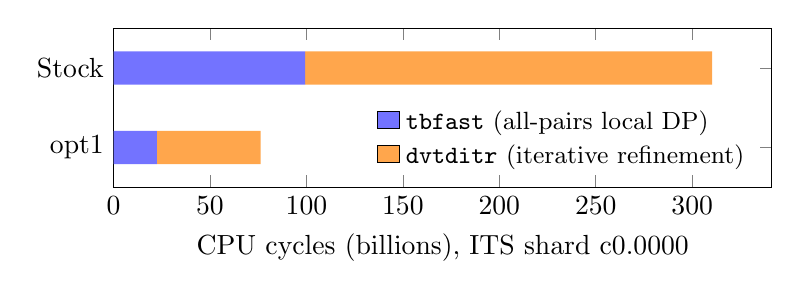
\begin{tikzpicture}
\begin{axis}[
  xbar stacked, width=0.82\linewidth, height=3.6cm,
  xlabel={CPU cycles (billions), ITS shard c0.0000},
  symbolic y coords={opt1,Stock}, ytick=data,
  bar width=12pt, xmin=0,
  legend style={at={(0.98,0.05)},anchor=south east,font=\small,draw=none,fill=none},
  legend cell align=left, enlarge y limits=0.5,
]
\addplot[fill=blue!55,draw=none] coordinates {(99.3,Stock) (22.4,opt1)};
\addplot[fill=orange!70,draw=none] coordinates {(211.0,Stock) (53.9,opt1)};
\legend{\code{tbfast} (all-pairs local DP), \code{dvtditr} (iterative refinement)}
\end{axis}
\end{tikzpicture}
\caption{Where the L-INS-i cycles went, stock and opt1.}
\end{figure}

The opt1 wall-clock benchmarks (Table~\ref{tab:wall}) compared Homebrew's stock MAFFT 7.526
with that build, on a machine whose only other load was macOS background services (load
average about 4). Every output from both builds was byte-identical to the pipeline's stored
reference alignments.

\begin{table}[h]
\centering
\caption{opt1 wall-clock time, L-INS-i on production ITS shards, \code{-{}-thread 1}.}
\label{tab:wall}
\begin{tabular}{lrrr}
\toprule
Test & Stock 7.526 & opt1 & Speedup \\
\midrule
8 shards, one at a time (total) & 717.9\,s & 186.9\,s & 3.84$\times$ \\
\quad per shard & 74--104\,s & 19--28\,s & 3.71--4.08$\times$ \\
16 shards, 8 concurrent (production setting) & 355.9\,s & 95.2\,s & 3.74$\times$\,$^\dagger$ \\
\bottomrule
\multicolumn{4}{l}{\footnotesize $^\dagger$Load rose during the stock run, so this ratio is
approximate; it agrees with the single-run ratio.}
\end{tabular}
\end{table}

The pipeline's own back-to-back measurements gave 3.56--3.97$\times$.

Table~\ref{tab:wall4} gives the current state, measured on macOS 27 with the same method:
builds alternated shard by shard for single runs, and batch order was alternated at 8-way
concurrency, where we also sampled the CPU used by all other processes and would have
discarded any batch run under significant outside load.

\begin{table}[h]
\centering
\caption{opt4 against stock 7.526 and against opt3, L-INS-i on r2 ITS shards,
\code{-{}-thread 1}, macOS 27. All outputs byte-identical to the stored references.}
\label{tab:wall4}
\begin{tabular}{lrrr}
\toprule
Test & Baseline & opt4 & Ratio \\
\midrule
\multicolumn{4}{l}{\emph{vs.\ stock Homebrew 7.526}} \\
8 shards one at a time, wall & 723.8\,s & 111.7\,s & 6.5$\times$ \\
\quad CPU time & 719.6\,s & 99.3\,s & 7.2$\times$ \\
16 shards 8 concurrent, wall & 285.7\,s & 62.6 / 61.3\,s & 4.6$\times$ \\
\quad CPU time & 2{,}021\,s & 310 / 336\,s & 6.3$\times$ \\
\midrule
\multicolumn{4}{l}{\emph{vs.\ opt3}} \\
8 shards one at a time, wall & 120.6\,s & 113.8\,s & 1.06$\times$ \\
\quad CPU time & 103.4\,s & 102.0\,s & 1.01$\times$ \\
16 shards 8 concurrent, wall & 64.5 / 69.9\,s & 63.3 / 66.9\,s & within noise \\
\bottomrule
\end{tabular}
\end{table}

The gain at 8-way concurrency is smaller than for single runs: the eight processes share one
GPU, half the M1's cores are efficiency cores, and short jobs make a 16-shard batch more
sensitive to how the last few line up. opt4's advantage over opt3 is marginal on this
workload; its GPU stage is faster, but that stage is now a small part of each run. Because
every build is byte-identical, choosing among them is purely a performance question.

At production concurrency a region of 2{,}415 shards now takes about 2.6 hours rather than
the roughly 12 it takes with stock MAFFT at the same concurrency.

opt8 brought the M1 code that the other platforms had developed (Section~\ref{sec:opt8}). Six
shards run singly, each once per build in two interleaved rounds, took 1{,}059.6\,s with Homebrew's
stock 7.526 and 131.5\,s with opt8: 8.1$\times$ in wall time and 9.2$\times$ in CPU time, with all 24
outputs identical to the stored references. At the production setting, the 16 shards of
Table~\ref{tab:wall4} at 8 concurrent, interleaved with stock and opt4 in two rounds with the
order reversed in the second, took 332\,s with stock, 76\,s with opt4 and 65.5\,s with opt8 (CPU
time 2{,}243, 425 and 354\,s): 5.1$\times$ over stock in wall time and 6.3$\times$ in CPU time, and
1.16$\times$ over opt4, with all 96 outputs identical to the references. Background load from the
OS was higher than in Table~\ref{tab:wall4} (other processes used 0.6--1.4 cores, more during the
optimized batches than during stock), so opt4's ratio came out at 4.4$\times$ rather than
4.6$\times$.

\subsection{x86}

The x86 benchmarks used the same discipline as on the M1, with nothing else running on the
instance: builds alternated shard by shard for single runs and batch by batch for concurrent
runs, and a sampler recorded any other CPU use. Production packs four single-threaded
alignments per 4-vCPU instance, so concurrency was four. Table~\ref{tab:x86} gives the
first clean comparison of the gcc builds on the c7i.

\begin{table}[h]
\centering
\caption{opt5 against stock 7.526, both built with gcc, on a c7i.xlarge; L-INS-i,
\code{-{}-thread 1}. All outputs byte-identical to stock.}
\label{tab:x86}
\begin{tabular}{lrrr}
\toprule
Test & Stock & opt5 & Ratio \\
\midrule
4 shards one at a time, total & 328.4\,s & 57.2\,s & 5.75$\times$ \\
\quad per shard & 75--98\,s & 12.0--17.3\,s & \\
16 shards, 4 concurrent & 595 / 589\,s & 106 / 104\,s & 5.6$\times$ \\
\quad throughput & 97 shards/h & 549 shards/h & \\
\midrule
\multicolumn{4}{l}{\emph{All 183 test shards, 4 concurrent, mean wall per shard}$^\dagger$} \\
\quad production shards & 157.6\,s & 28.2\,s & 5.6$\times$ \\
\quad targeted windows (217--532 seqs) & 541\,s & 92.7\,s & 5.8$\times$ \\
\quad current-build shards & 107.5\,s & 21.1\,s & 5.1$\times$ \\
\bottomrule
\multicolumn{4}{l}{\footnotesize $^\dagger$The stock run shared the machine with builds at times,
so its times are slightly inflated.}
\end{tabular}
\end{table}

Table~\ref{tab:x86four} compares all four builds on both instance types, each set measured
within one session. The c7i ran 8--15\% slower in its second session than in its first (the
same opt5 batch took 121\,s against 104--106\,s), presumably for host-level reasons, so builds
are compared only within a session. On both machines clang+FMA is 2--6\% faster than gcc,
for stock and for opt5.

\begin{table}[h]
\centering
\caption{Four builds on two instance types, L-INS-i, \code{-{}-thread 1}: 16 production
shards at 4 concurrent (batch wall time, and throughput), and two shards run singly
(c0.0016 / c0.0017). Every output matched the stock build of the same rounding.}
\label{tab:x86four}
\begin{tabular}{lrrrr}
\toprule
& \multicolumn{2}{c}{Stock 7.526} & \multicolumn{2}{c}{opt5} \\
\cmidrule(lr){2-3}\cmidrule(lr){4-5}
& gcc & clang+FMA & gcc & clang+FMA \\
\midrule
\multicolumn{5}{l}{\emph{c7i.xlarge (2 cores $\times$ 2 hyperthreads)}} \\
16 shards, 4 concurrent & 639\,s & 601\,s & 121\,s & 117\,s \\
\quad throughput (shards/h) & 90 & 96 & 476 & 492 \\
single runs & 82.0 / 108.6\,s & 79.1 / 104.1\,s & 13.4 / 19.3\,s & 13.3 / 18.8\,s \\
\midrule
\multicolumn{5}{l}{\emph{c7a.xlarge (4 cores)}} \\
16 shards, 4 concurrent & 439\,s & 411\,s & 76\,s & 70\,s \\
\quad throughput (shards/h) & 131 & 140 & 758 & 823 \\
single runs & 88.0 / 130.5\,s & 82.8 / 124.9\,s & 12.9 / 18.1\,s & 12.4 / 17.2\,s \\
\bottomrule
\end{tabular}
\end{table}

Single-threaded speed is similar on the two machines: opt5 is slightly faster on the c7a and
stock slightly slower. The c7a's advantage is its four real cores: four concurrent jobs
barely slow each other there, whereas on the c7i two hyperthreads share each core and four
jobs give only about 2.2--2.3 times the throughput of one (approximate, since the single runs
and the batches used different production shards). Over all 183 test shards at four concurrent, opt5-clang took 1{,}082\,s on the c7a and
1{,}845\,s on the c7i. At us-west-2 prices at the time (on-demand \$0.205/h for c7a.xlarge and
\$0.1785/h for c7i.xlarge), opt5-clang costs about \$0.25 per 1{,}000 shards on the c7a and
\$0.33--0.36 on the c7i; at a week's range of Spot prices, \$0.11--0.15 and \$0.12--0.20.
The deployment uses the c7a, with the c7i as a Spot fallback, since the two give identical
output. For comparison, opt4 on the M1 aligns about 930 shards per hour at 8 concurrent.

\subsection{Across architectures}
\label{sec:allarch}

Table~\ref{tab:allarch} collects the current speedups over stock. The same 16 shards and two
singles were used throughout, with batch order alternated and a sampler watching for outside
load, as above. Where opt8 was not run on a machine, the table gives opt7.

\begin{table}[h]
\centering
\caption{Speedup over stock 7.526 built the same way on the same machine, L-INS-i on production
ITS shards, \code{-{}-thread 1} per run: 16 shards at four concurrent and two shards run singly
(on the M1: 8 concurrent, and six shards singly).}
\label{tab:allarch}
\begin{tabular}{llrr}
\toprule
Machine & Build & 16 shards, 4 concurrent & Single runs \\
\midrule
Apple M1, with the Metal GPU & opt8 & 5.1$\times$$^\ddagger$ & 8.1$\times$ \\
c7a (Zen 4), clang+FMA & opt8 & 8.6$\times$$^*$ & 10.5$\times$$^*$ \\
c7i (Sapphire Rapids), clang+FMA & opt8 & 7.5$\times$$^*$ & 8.1$\times$$^*$ \\
c8a (Zen 5), clang+FMA & opt7 & 9.8$\times$ & 12.2$\times$ \\
c8i (Granite Rapids), clang+FMA & opt7 & 8.2$\times$ & 9.3$\times$ \\
c8g (Graviton4), clang & opt8 & 5.0$\times$$^*$ & 5.6$\times$$^*$ \\
c7g (Graviton3), clang & opt7 & 5.1$\times$ & 5.6$\times$ \\
g6 (L4 + Zen 3 host), clang+FMA, CUDA & opt8 & 8.0$\times$$^\dagger$ & 9.6$\times$$^\dagger$ \\
\quad the same without CUDA & opt8 & 6.5$\times$$^\dagger$ & 7.6$\times$$^\dagger$ \\
Zen 3 host, AVX2 only, gcc & opt8 & 5.9$\times$ & 7.1$\times$ \\
\quad FFT-NS-i (\code{-{}-maxiterate 1000}) & opt8 & 2.6$\times$ & \\
\bottomrule
\multicolumn{4}{l}{\footnotesize $^*$Stock timed on the same instance type in an earlier session (Table~\ref{tab:x86four}; Table~\ref{tab:opt7} for c8g).}\\
\multicolumn{4}{l}{\footnotesize $^\dagger$Against stock built with gcc, which is 2--6\% slower than stock built with clang.}\\
\multicolumn{4}{l}{\footnotesize $^\ddagger$At 8 concurrent, the production setting on the M1.}
\end{tabular}
\end{table}

Cross-session ratios carry the drift noted above: the c7i ran up to 15\% slower in one session
than another, while on the c8g opt7 timed in two sessions agreed within 1\%. On the L4 instance
the GPU added 1.24$\times$ to opt8 and was idle in most five-second samples: the refinement, which
stays on the CPU, dominates. At on-demand prices that is about \$1.10 per 1{,}000 shards, against
about \$0.17 on a c7a with opt8 and \$0.11 on a c8a with opt7.

\section{What did not work, and limitations}

\begin{itemize}
\item \textbf{Generality.} The speedups, not the exactness, are specific to this workload and
  hardware. Which optimizations paid depended on the shape of the alignments (about 180
  sequences, about 2{,}000 columns, 71\% gaps), on the default scoring settings, and on the
  machine: banding the importance matrix did not help with a 105\,MB L3 but did with Graviton's
  small L2, a GPU pays on the M1 but not on AWS, and gains at four concurrent ranged from
  about 5$\times$ on Graviton to nearly 10$\times$ on Zen~5. Other inputs or machines may see smaller gains. Every
  fast path checks its preconditions and falls back to the original code, so they will see
  the same output.
\item \textbf{Blocked prefix scan.} Splitting the \code{L\_\_align11} row scan into four
  interleaved chains followed by a fix-up pass was slower when measured side by side
  (28.6G vs.\ 39.2G \code{tbfast} cycles, the latter being the blocked version), and was
  reverted. The added pass and branches cost more than the extra parallelism gained.
\item \textbf{Other scan variants} (Section~\ref{sec:round2}): a scalar next-row scan fused into
  the vector loop, and a two-block unrolled vector scan, were slower or no faster.
\item \textbf{Whole-step memoization in refinement} could reuse at most 2\% of steps, and a
  cache of anchor profiles across FFT lags turned out never to run, since L-INS-i and
  FFT-NS both use MAFFT's single-lag anchoring mode. Both were dropped.
\item \textbf{GPU variant tuning}: finer column-count variants gave nothing; register-resident
  state was a net loss (Table~\ref{tab:occupancy}).
\item \textbf{Scope.} The integer and zero-extension fast paths apply to the default
  scoring settings. Non-default settings, such as fractional \code{-{}-consweight},
  nonzero \code{-{}-gexp} in progressive modes, or \code{-{}-allowshift}, take the original
  code, and are exact but not faster.
\item \textbf{Threads.} We did not make \code{-{}-thread N} deterministic. Stock MAFFT is
  already nondeterministic there, and the pipeline parallelizes across inputs instead.
\item \textbf{Platforms.} All feature tests are in \code{core/mafft\_simd.h}. Apple silicon,
  Linux arm64 (Graviton3 and 4), x86-64 with AVX-512 (Zen~4 and~5, Sapphire Rapids, Granite
  Rapids) and with AVX2 only (Zen~3, and the Broadwell Dikarya host for dikarya1), and NVIDIA L4
  and T4 GPUs were verified. Other targets compile the same algorithms in scalar code, which is
  exact by construction but was not benchmarked; opt8 has not yet been timed on the Dikarya host.
\item \textbf{Ideas that did not pay} in opt7 and opt8: a 16-lane marker fill (no gain on Zen~4 or
  Sapphire Rapids; 6\% on Zen~5, then superseded); fills storing flag bits instead of the
  traceback; tracking the row maximum inside the fill loop; a gather/scatter importance-matrix
  walk; AMX; a NEON prefix scan in the profile-DP rows; SVE on 128-bit vectors; and, on Graviton,
  per-character byte masks and the portable popcount pair scores, which opt8 had to take back
  (Section~\ref{sec:opt8}).
\item \textbf{GPU on AWS.} The CUDA stage is exact and adds about 1.2$\times$, but on the GPU
  instances available the refinement on few CPU cores dominates, and the cost per alignment was
  more than ten times that of a CPU-only instance. Refinement was not moved to the GPU: it runs
  step by step in double precision, which the L4 executes at about 1/64 of its single-precision
  rate.
\item \textbf{Parallel agents.} One agent let its results be lost by waiting on a job past its
  instance's fixed lifetime, and the coordinating session did not check on it in time; later
  runs copied results back after every step. Merged parallel work was a union rather than a
  design until it was consolidated (Section~\ref{sec:convergence}).
\item \textbf{Version strings.} The version string does not record the rounding class, so a gcc
  and a clang+FMA build of the same commit cannot be told apart by it
  (Section~\ref{sec:provenance}).
\item \textbf{Trees.} The tree stage is not reproducible across platforms or FastTree builds
  (Section~\ref{sec:xplat}). We did not try to make it so: that would mean building FastTree
  without \code{-funsafe-math-\allowbreak optimizations} on every platform, and would still leave
  differences between the math libraries.
\item \textbf{Coverage.} The corpus the pipeline now aligns on AWS includes ITS sequences up to about
  3{,}000\,bp, longer than anything in the test sets. Those exercise the same code but will cost
  more per shard than the timings here suggest.
\item \textbf{GPU limits.} The GPU takes second sequences of 64--2{,}048 residues; others use
  the CPU. If the embedded shader library fails to load, opt4 silently falls back to
  compiling the source; the only sign is a line on standard error, which MAFFT's
  \code{-{}-quiet} discards.
\end{itemize}

\section{Conclusions}

Mature scientific code can hold large, exact speedups: here 8.1$\times$ on the M1 and
5--10$\times$ on AWS CPUs, mostly from bookkeeping and data layout rather than new algorithms,
and without changing an output byte, so nothing downstream had to be revalidated. Porting
showed that ``identical to stock'' must name the stock build, because the compiler's rounding
of multiply-adds alone changed a third of the alignments between platforms.

The later builds tried a way to extend this work across hardware. Three agents, each with its
own machines and the same contract, produced verified speedups for three architectures in
parallel, each within about seven hours. Working from the same tree and the same profile without
communicating, they reached several of the same exact transformations, which suggests these are
natural ones for this code rather than one agent's habits. Merged as written, however, their work
was a union: the same ideas in per-platform copies, each run and tested only where it was born.
Consolidating them into portable code with small per-platform primitives made the code smaller,
put each technique under test on every platform, and made every platform we measured faster,
since each gained what the others had found. It also needed measurement before sharing, as the Graviton
regression showed. The parallel phase found the ideas; the consolidation spread them.

The broadening began with Alan Rockefeller's dikarya1 work for Dikarya's AVX2 server. It
contributed the marker fill, which made our own x86 production build faster, and it
prompted us to explore more architectures, which paid off on every platform we measured,
including the M1 where the series began.

This work was done by an AI coding agent, Claude Code running Claude Opus 5.5, with a
researcher setting the direction and the acceptance rules. The first five builds took about a
week of calendar time, and dikarya1's evaluation through opt8 about a day and a half more,
within a \$200/month subscription; by the authors' estimate the same work would have taken a
human developer several weeks. AWS instances for opt7 and opt8 cost on the order of \$25 (our
estimate; costs were not recorded per instance). The compute savings alone repay the
subscription slowly: at on-demand prices opt8 on a c7a saves about \$1.29 per 1{,}000 shards
(\$1.46 against \$0.17), so even charging a whole month to this work, it is recouped only after
about 155{,}000 shards, roughly 65 regions. The immediate return is turnaround: a region that
took about 12 hours to align on the M1 with stock MAFFT now takes about 2.6 hours with opt4,
and less with opt8.

What made the work safe to delegate was verification, not the agent. The exactness contract
was fixed in advance, each rewritten function was checked against the original on every call,
object-file comparison showed which targets a change could affect, so that verification
carried over across merges and refactors, and a separate Claude Code session working on the
pipeline, under its own user's approval, validated each Mac build on production data before it
was installed. The independent check caught the one error the rewrite introduced
(Section~\ref{sec:bug}).

For compute-bound pipelines that run a fixed tool at scale, we therefore recommend profiling
the dominant tool on the hardware it actually runs on and, where results must not change,
attempting exact optimization under the same discipline: an explicit output contract,
per-function bitwise checks, and validation by someone other than the author of the change.
Where several platforms matter, parallel per-platform work is effective, provided it is
followed by a deliberate consolidation.

\section{Related work}

SIMD acceleration of pairwise DP is well established. It includes anti-diagonal
vectorization~\cite{wozniak1997}, Farrar's striped layout~\cite{farrar2007}, inter-sequence
parallelism~\cite{rognes2011}, and general libraries such as parasail~\cite{daily2016}.
Those methods typically target score-only or database-search settings with standard
affine recurrences. Our case differs in two ways. First, we must reproduce MAFFT's own
recurrence and traceback conventions and its floating-point rounding exactly. Second, the
largest wins came from removing redundant bookkeeping and from recasting reductions as
dense matrix products that run on matrix hardware. Faster DP kernels alone would not have
produced them. GPU implementations of Smith--Waterman are likewise established, usually for database search
with score-only kernels; our kernel instead computes MAFFT's own recurrence and full
traceback, bit-exactly, for all pairs of a set. Approximate alternatives, such as faster MAFFT modes or other
aligners~\cite{vaser2017}, trade accuracy for speed. The downstream measurements cited
in the introduction quantify that trade for this workload. That floating-point results
depend on compiler contraction and optimization flags is well known in principle; what we
add is a measurement of its size for one widely used aligner on real data (a third of
inputs) and a demonstration that matching the contraction rule alone restores identical
output across architectures.

\section{Availability and future work}
\label{sec:avail}

The builds are a linear series of commits on top of upstream GitLab \code{main} (7.526,
including December 2025 commits). They are published, with this report, as the
\code{exact-speedups} branch of an unofficial fork,
\url{https://github.com/joshuaowalker/mafft}, with one tag per build (\code{v7.526-opt1} to
\code{v7.526-opt8}, and \code{v7.526-opt5-dikarya1}). opt8 changes 23 files (+5{,}052/$-$302
lines), all in \code{core/}; the feature tests are in \code{core/mafft\_simd.h}, and the fork's
README gives the build flags for each platform. The per-call harnesses are in the fork's
\code{harness/} directory as patch scripts, one directory per build that introduced them, with
the object-file comparison script beside them. opt4 is installed for local projects on the Mac;
on AWS, opt5 runs in a container image built from these sources (clang 15 with \code{-O3
-march=x86-64-v4 -DMAFFT\_STOCK\_FMA=1}), next to the clang+FMA stock reference, trimAl 1.5.1,
and the bioconda FastTree binary, copied rather than rebuilt. A self-contained canary checks a
build in one command: L-INS-i on the 13 canary windows and the 12 placement cases against the
Mac's stored outputs, plus the tree stage against x86 hashes. Its alignment checks pass on every
build since opt4 on the M1 and on every AWS machine above, and it fails on exactly the five divergent windows when given a gcc
build. The canary is built from the pipeline's data and is not published.

Promising next steps are:
(i)~timing opt8 on the Dikarya host itself;
(ii)~moving the AWS deployment to opt8, which with the same flags is 1.35$\times$ faster than opt6
and opt7 (and more than the deployed opt5), or to a c8a;
(iii)~trying the striped fill at 8 and 4 lanes for AVX2 and NEON, and the end-cell search in the
striped fill;
(iv)~recording the rounding class in the version string itself;
(v)~making the shader fallback observable, or optionally an error;
(vi)~testing the longest ITS sequences the pipeline now aligns;
and (vii)~offering these changes to the MAFFT maintainers.

\section*{Acknowledgments}

We thank Alan Rockefeller, who directed the dikarya1 work for Dikarya and made it public. His
marker fill made our own builds faster, and his work prompted the multi-architecture
exploration of opt7 and opt8, which paid off on every platform we measured.

\begin{thebibliography}{99}\small
\bibitem{katoh2002} K.~Katoh, K.~Misawa, K.~Kuma, T.~Miyata. MAFFT: a novel method for
  rapid multiple sequence alignment based on fast Fourier transform.
  \emph{Nucleic Acids Res.} 30:3059--3066, 2002.
\bibitem{katoh2005} K.~Katoh, K.~Kuma, H.~Toh, T.~Miyata. MAFFT version 5: improvement in
  accuracy of multiple sequence alignment. \emph{Nucleic Acids Res.} 33:511--518, 2005.
\bibitem{katoh2013} K.~Katoh, D.~M.~Standley. MAFFT multiple sequence alignment software
  version 7: improvements in performance and usability. \emph{Mol. Biol. Evol.}
  30:772--780, 2013.
\bibitem{price2010} M.~N.~Price, P.~S.~Dehal, A.~P.~Arkin. FastTree 2 -- approximately
  maximum-likelihood trees for large alignments. \emph{PLoS ONE} 5:e9490, 2010.
\bibitem{capella2009} S.~Capella-Guti\'errez, J.~M.~Silla-Mart\'inez, T.~Gabald\'on.
  trimAl: a tool for automated alignment trimming in large-scale phylogenetic analyses.
  \emph{Bioinformatics} 25:1972--1973, 2009.
\bibitem{vaser2017} R.~Vaser, I.~Sovi\'c, N.~Nagarajan, M.~\v{S}iki\'c. Fast and accurate
  de novo genome assembly from long uncorrected reads. \emph{Genome Res.} 27:737--746,
  2017.
\bibitem{wozniak1997} A.~Wozniak. Using video-oriented instructions to speed up sequence
  comparison. \emph{Comput. Appl. Biosci.} 13:145--150, 1997.
\bibitem{farrar2007} M.~Farrar. Striped Smith--Waterman speeds database searches six times
  over other SIMD implementations. \emph{Bioinformatics} 23:156--161, 2007.
\bibitem{rognes2011} T.~Rognes. Faster Smith--Waterman database searches with
  inter-sequence SIMD parallelisation. \emph{BMC Bioinformatics} 12:221, 2011.
\bibitem{daily2016} J.~Daily. Parasail: SIMD C library for global, semi-global, and local
  pairwise sequence alignments. \emph{BMC Bioinformatics} 17:81, 2016.
\end{thebibliography}

\end{document}
